% called by main.tex
%
\chapter{Análisis inicial}
\label{ch::chapter3}

El objetivo de este capítulo es caracterizar el conjunto de datos y los prompts utilizados en el trabajo,
un análisis que muestre las tensiones estructurales del problema \citep{yang2025structeval, li2023strucbench}. El análisis inicial sirve para anclar las decisiones de 
diseño posteriores: explica por qué
ciertos modelos fallan de formas específicas, por qué ciertas métricas son necesarias y qué se observa en los experimentos.

Todos los manifiestos analizados aquí son \textit{canónicos}: han sido parseados, validados y serializados de forma determinista, partiendo del mismo tipo de pares
prompt--manifiesto que emplean benchmarks recientes de generación de YAML cloud-native \citep{xu2024cloudevalyaml, cloudeval2023}. El proceso seguido es simple: dado un
prompt en lenguaje natural, el modelo debe generar una secuencia de bloques estructurados (documento, índice de línea, nivel de indentación, texto) cuya
reconstrucción mediante indentación produce un manifiesto YAML válido. Esto supone ya que el YAML está normalizado.

\section{El conjunto de datos}

\subsection{Descripción general}

El dataset base está compuesto por 283 muestras que contienen un total de 338 manifiestos Kubernetes válidos. Cada muestra incluye dos variantes de prompt en lenguaje
natural: una descripción más elaborada y una versión simplificada. Esto suma un total de 566 pares prompt--manifiesto en la distribución de entrenamiento. El dataset se
divide en tres conjuntos: 213 muestras para entrenamiento, 35 para validación y 35 para evaluación final.

Un aspecto importante del preprocesado fue el control de fugas (\textit{leakage}). Se identificaron 51 muestras que contienen manifiestos exactamente duplicados, y
todas ellas fueron agrupadas en el mismo conjunto (siempre entrenamiento). Además, se detectaron 51 pares de prompts duplicados exactamente y aproximadamente 15 pares
con similitud mayor a 0.97, que también fueron agrupados para evitar que el modelo entrenara en una muestra y evaluara en su duplicado.

Cabe destacar que cada muestra se usa 2 veces. Por un lado aparece como objetivo del prompt más elaborado (question) y por otro como objetivo del prompt simplificado
(simplified).

\begin{table}[htbp]
\centering
\caption{Resumen cuantitativo del dataset canónico utilizado en este capítulo.}
\label{tab:ch3_dataset_summary}
\begin{tabular}{lr}
\toprule
\textbf{Magnitud} & \textbf{Valor} \\
\midrule
Muestras totales & 283 \\
Documentos Kubernetes totales & 338 \\
Pares prompt--manifiesto & 566 \\
Muestras de entrenamiento & 213 \\
Muestras de validación & 35 \\
Muestras de test & 35 \\
Muestras con YAML duplicado (agrupadas) & 51 \\
Pares de prompt duplicado exacto & 51 \\
Pares de prompt casi duplicado (similitud $>$ 0.97) & 15 \\
\bottomrule
\end{tabular}
\end{table}

\begin{figure}[htbp]
\centering
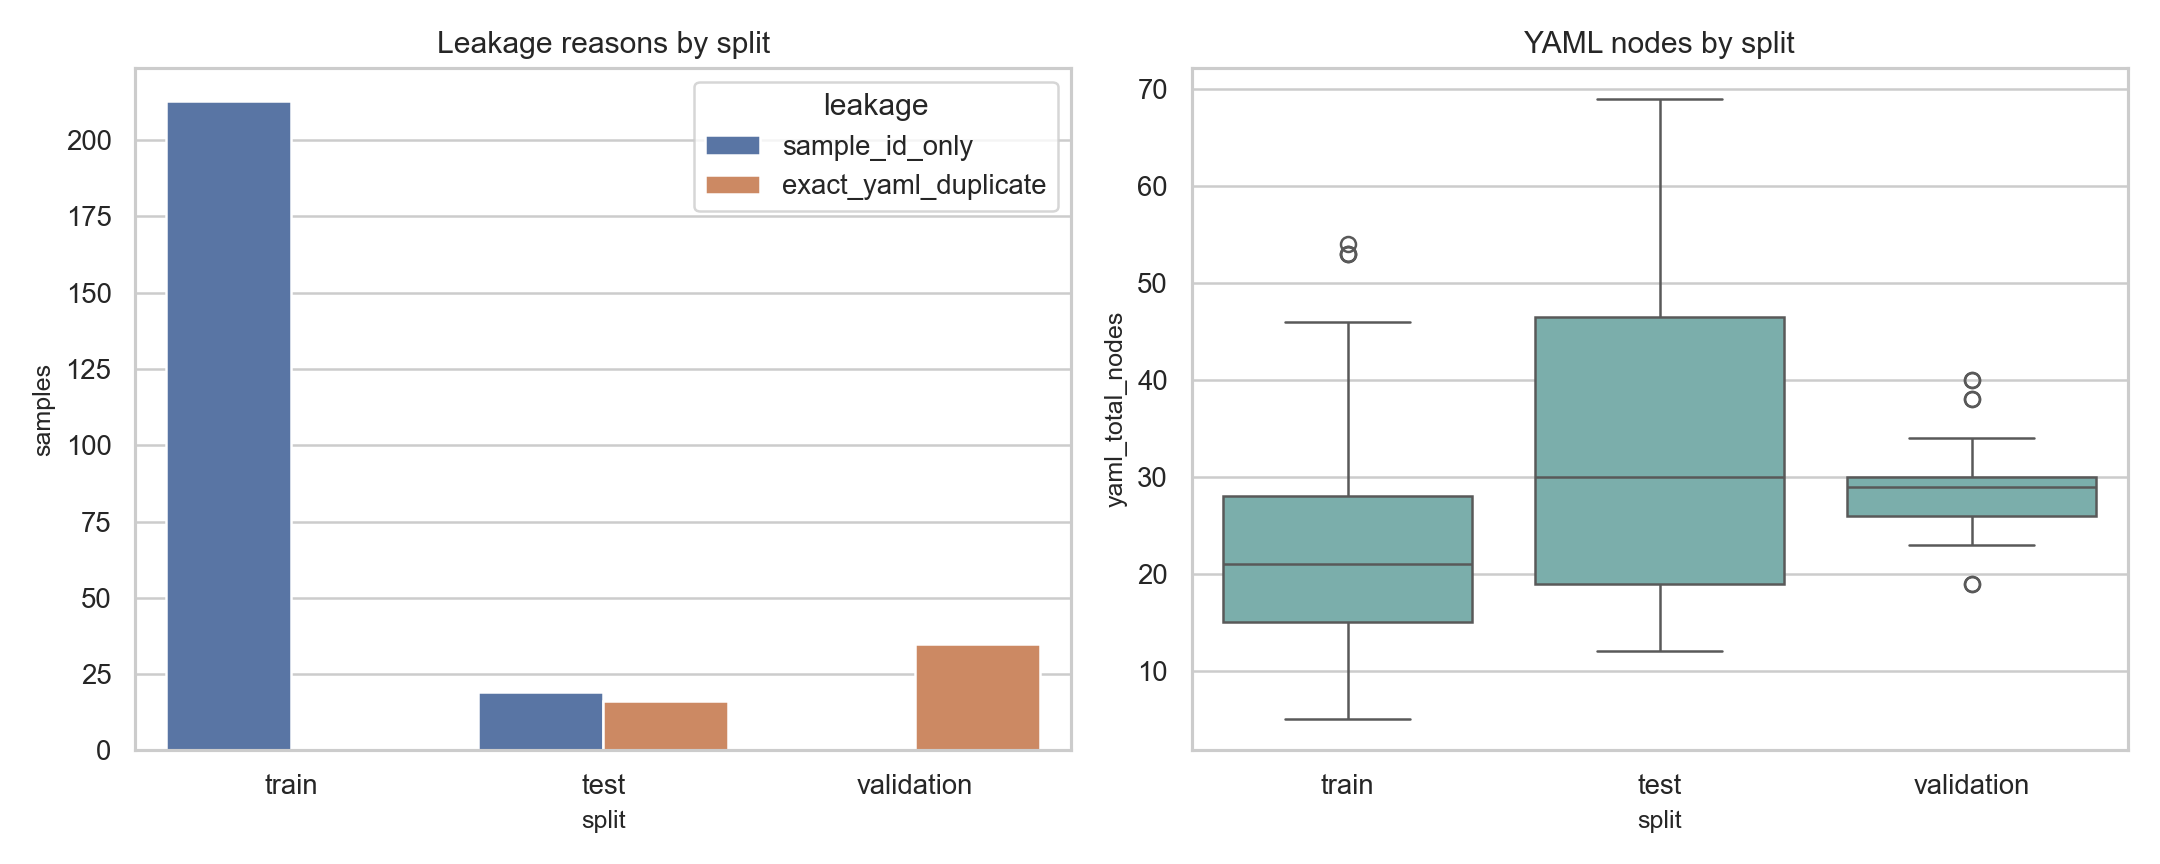
\includegraphics[width=0.82\textwidth]{figures/chapter3/split_balance_and_leakage.png}
\caption{Balance del dataset por split y control de fugas entre entrenamiento, validación y test.}
\label{fig:ch3_split_leakage}
\end{figure}

\subsection{Distribución de tipos de recurso}

Los manifiestos en el dataset corresponden a varios tipos de recursos Kubernetes (\textit{kinds}). La distribución no es uniforme. Los ocho tipos más frecuentes:
(Pod (56), DaemonSet (55), Service (31), Deployment (21), Job (20), PersistentVolume (16), Secret (14), StatefulSet (14)) representan aproximadamente el 64\% del
total de documentos. El resto distribuye entre tipos menos comunes: ConfigMap (12), ReplicaSet (9), Namespace (5), CronJob (4) y otros. Esta concentración tiene
implicaciones para el aprendizaje del modelo, no solo en términos de frecuencia sino de complejidad estructural, que se analiza más adelante.

La distribución de versiones de API refleja la variedad del ecosistema real de Kubernetes, un rasgo que se ve reflejado en estudios empíricos sobre configuraciones y defectos en manifiestos del dominio \citep{rahman2023securityk8s, zhang2025kubernetesdefects}: v1 (núcleo del API, 48\%), apps/v1 (workloads, 30\%), batch/v1 (tareas programadas, 8\%),
rbac.authorization.k8s.io/v1 (control de acceso, 6\%) y otras versiones. Por último, respecto a la estructura de los manifiestos, casi todas las muestras (238 de 283)
contienen un único recurso por manifiesto. Solo 36 muestras contienen dos recursos y 8 contienen tres.

\begin{figure}[htbp]
\centering
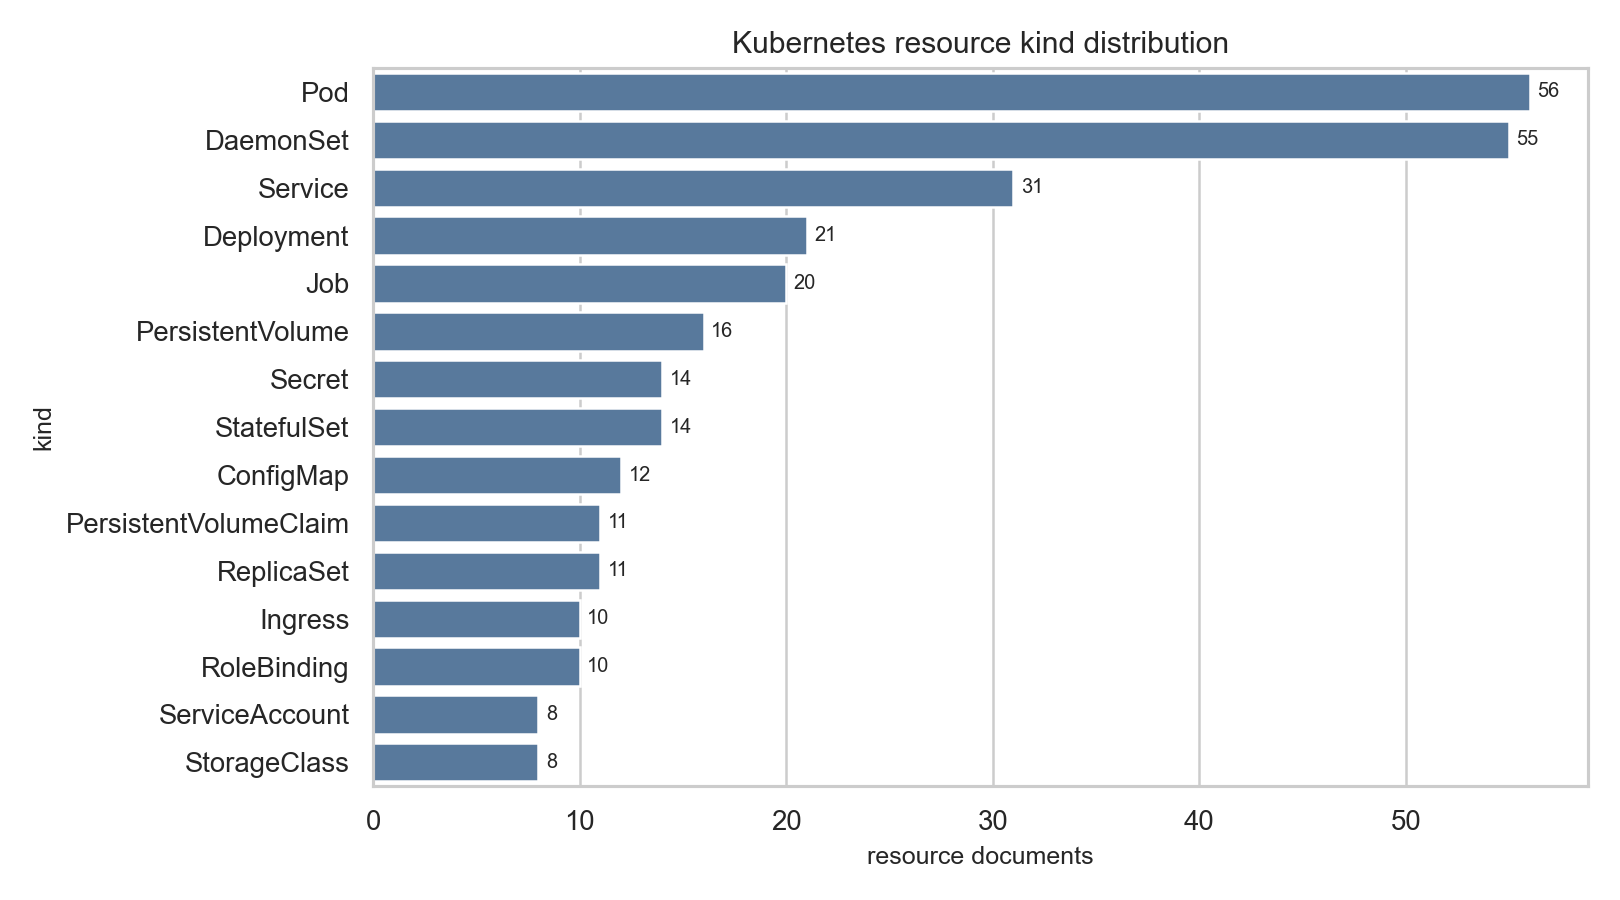
\includegraphics[width=0.78\textwidth]{figures/chapter3/kind_counts.png}
\caption{Distribución de \textit{kinds} en el corpus Kubernetes.}
\label{fig:ch3_kind_counts}
\end{figure}

\begin{figure}[htbp]
\centering
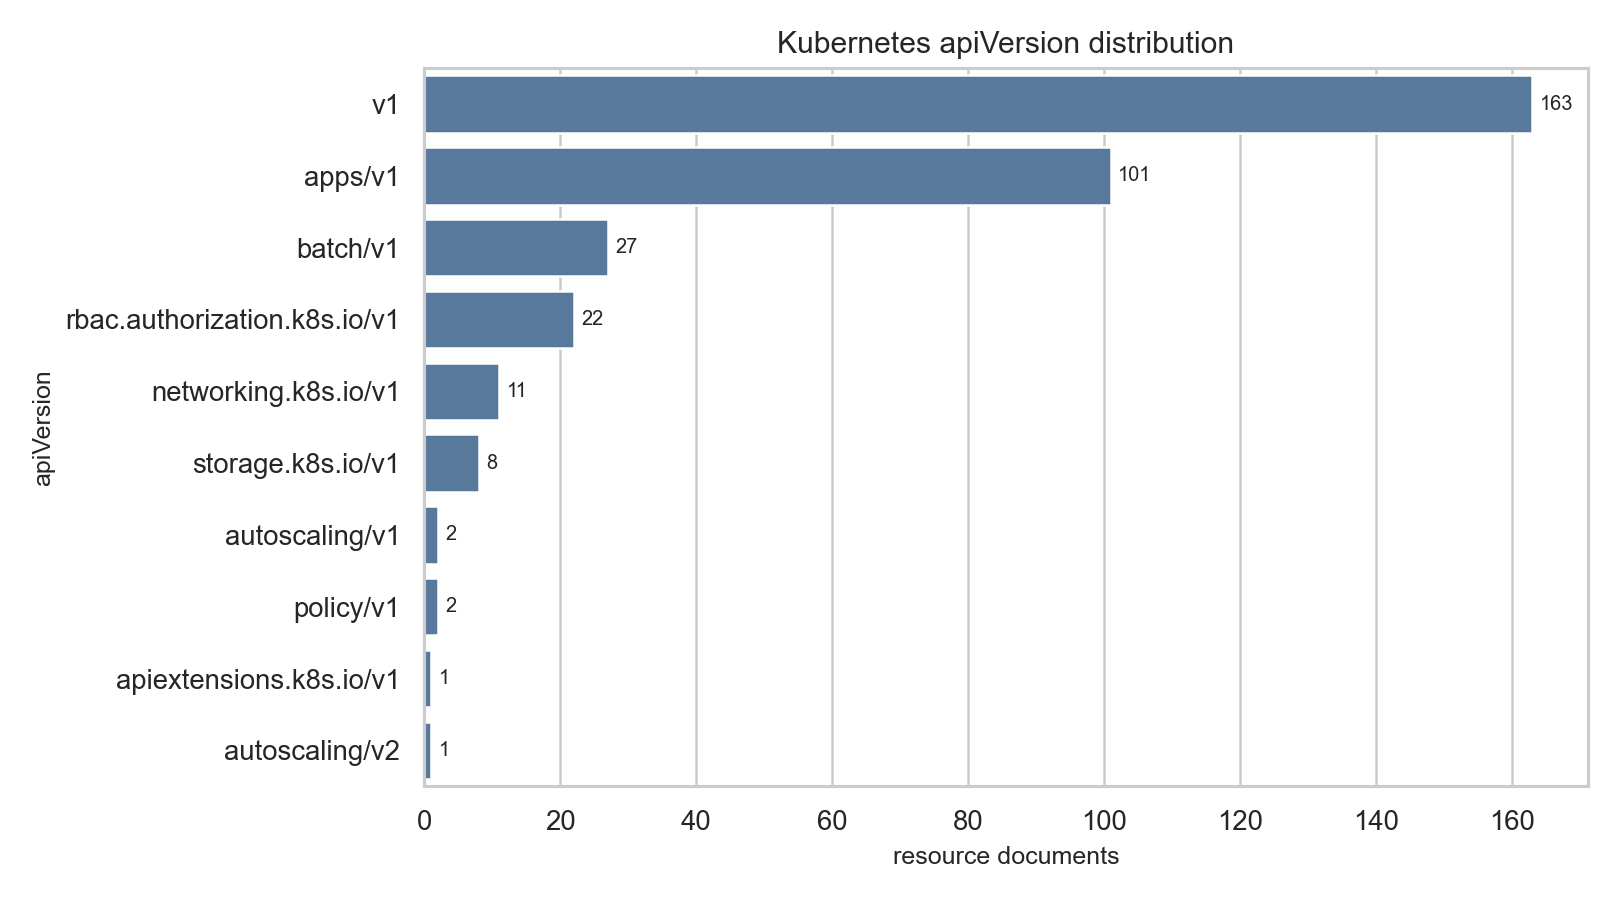
\includegraphics[width=0.78\textwidth]{figures/chapter3/api_version_counts.png}
\caption{Distribución de versiones de API en los manifiestos del dataset.}
\label{fig:ch3_api_versions}
\end{figure}

\section{Representación jerárquica: la secuencia nivel-línea}

\subsection{El contrato de estructura}

En este capítulo se usa la representación secuencia-nivel-línea como lente descriptiva para estudiar distribución de complejidad y patrones de dificultad. La
especificación formal del contrato de datos, la definición operacional de \texttt{document\_index}/\texttt{line\_index}/\texttt{level} y el pipeline de transformación
de YAML canónico a formato tabular se desarrolla de forma completa en el capítulo \ref{ch::chapter4}, sección \ref{sec:ch4_contract}.

\subsection{Estadísticas de profundidad y complejidad}

Las muestras del dataset presentan variaciones significativas en tamaño y profundidad. El número de líneas por manifiesto (\texttt{block\_count}) varía desde un mínimo
de 4 líneas hasta un máximo de 59, con mediana de 20 líneas. Esto refleja la heterogeneidad de los manifiestos: algunos son objetos de configuración simples (como un
ConfigMap con unos pocos pares clave-valor), mientras que otros son deployments complejos con especificaciones de plantillas, volúmenes y selectores.

La profundidad máxima de indentación por muestra (\texttt{max\_block\_level}) también varía considerablemente, con mínimo de 3, percentil 75 en 9 y máximo de 13.
Esto significa que algunos manifiestos tienen anidamiento profundo (caso típico: Deployment con spec \(\rightarrow\) template \(\rightarrow\) spec \(\rightarrow\) containers),
mientras que otros permanecen en niveles superficiales.

Pero el rasgo más importante es la \textit{distribución de niveles en el conjunto completo de bloques}. Si \(N_b\) denota el número total de bloques y \(\ell_i\)
el nivel del bloque \(i\), la proporción de bloques en cada nivel \(k\) puede definirse como:

\[
p_k = \frac{1}{N_b}\sum_{i=1}^{N_b}\mathbf{1}[\ell_i = k].
\]

Esta definición permite separar la intuición visual de la figura de una magnitud concreta: cuando contamos cuántos bloques del dataset completo caen en
cada nivel de indentación, emerge un patrón claro:

\begin{itemize}
\item Nivel 0: 1.443 bloques (primeras claves del manifiesto: \texttt{apiVersion}, \texttt{kind}, \texttt{metadata}, \texttt{spec})
\item Nivel 1: 1.541 bloques (contenido de \texttt{metadata} y \texttt{spec})
\item Nivel 2: 1.045 bloques (subestructuras como \texttt{labels}, \texttt{selector}, \texttt{containers})
\item Nivel 3: 818 bloques
\item Nivel 4: 796 bloques
\item Nivel 5: 232 bloques (7.8\% del total)
\item Nivel 6: 153 bloques (4.5\%)
\item Niveles 7 - 8: 45 bloques combinados (1.5\%)
\end{itemize}

\begin{table}[htbp]
\centering
\caption{Distribución de bloques por nivel de indentación.}
\label{tab:ch3_level_distribution}
\begin{tabular}{lrr}
\toprule
\textbf{Nivel} & \textbf{Bloques} & \textbf{Porcentaje} \\
\midrule
0 & 1.443 & 23.8\% \\
1 & 1.541 & 25.4\% \\
2 & 1.045 & 17.2\% \\
3 & 818 & 13.5\% \\
4 & 796 & 13.1\% \\
5 & 232 & 3.8\% \\
6 & 153 & 2.5\% \\
7 - 8 & 45 & 0.7\% \\
\bottomrule
\end{tabular}
\end{table}

\begin{figure}[htbp]
\centering
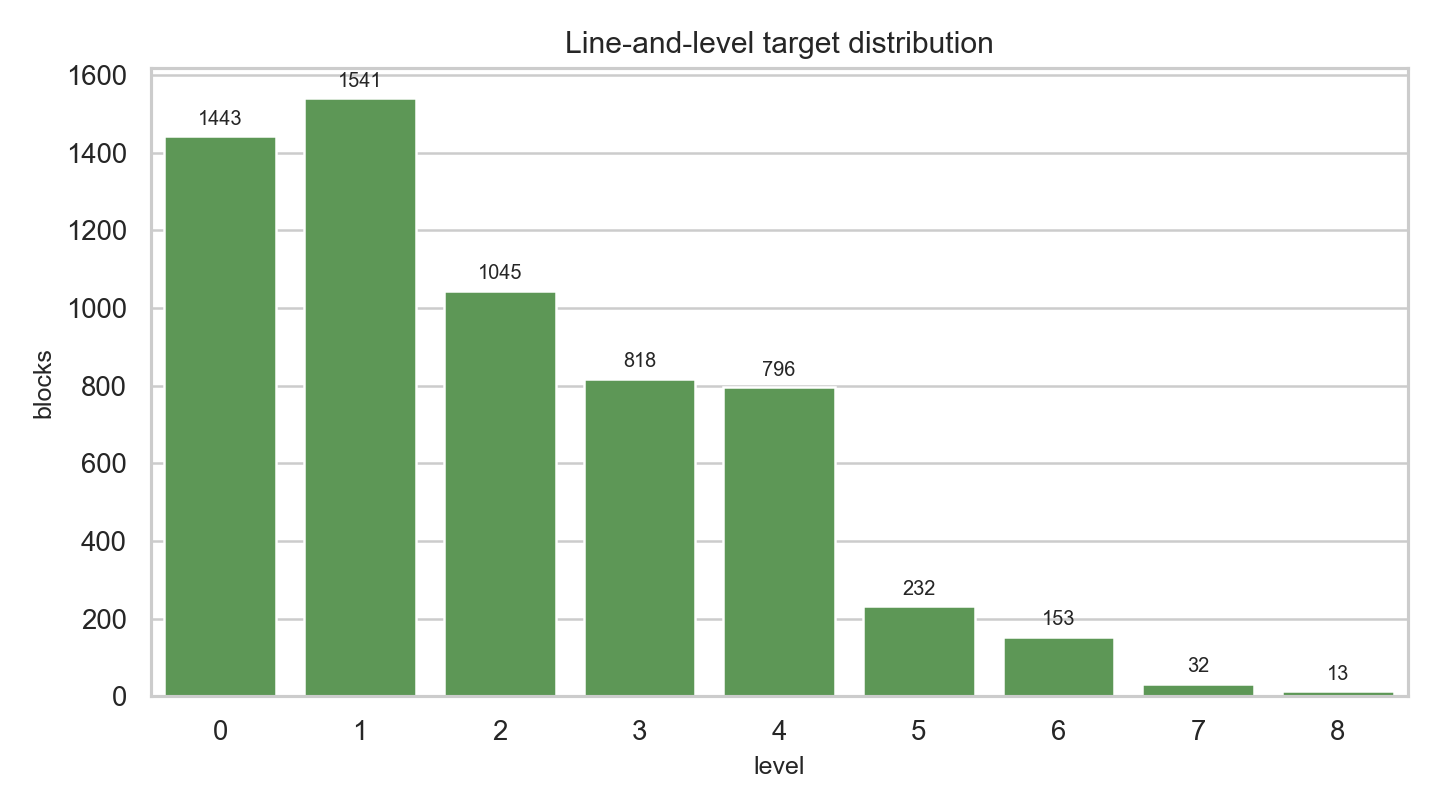
\includegraphics[width=0.78\textwidth]{figures/chapter3/level_distribution.png}
\caption{Distribución de bloques por nivel de indentación en el conjunto canónico.}
\label{fig:ch3_level_distribution}
\end{figure}

\noindent Existe un \textit{desbalanceo severo} hacia niveles bajos. A partir del nivel 5, la cantidad de ejemplos cae de forma brusca. Este hecho tiene implicaciones
directas para el aprendizaje: un modelo que intenta predecir \texttt{level} como un número dentro de una secuencia tiene muy pocos ejemplos de niveles profundos y,
por tanto, poco incentivo para aprender a predecirlos correctamente.

Precisamente en este punto se introdujo un experimento diagnóstico previo al entrenamiento estructural. Su objetivo fue verificar 
una pregunta metodológica más básica: si los estados ocultos del modelo base ya contienen señal recuperable sobre la variable \texttt{level}, siguiendo
la intuición de los trabajos de \textit{structural probing} sobre representaciones internas de modelos de lenguaje \citep{hewitt2019structural, clark2019bert}. En este sentido, 
el experimento actúa como una comprobación de factibilidad para la hipótesis estructural del trabajo.

Formalmente, el experimento puede verse como un clasificador ligero que intenta reconstruir el nivel jerárquico a partir de un estado oculto del modelo:

\[
\hat{\ell}_i = g_\phi(h_i),
\]

donde \(h_i\) es la representación latente asociada a la línea \(i\), \(g_\phi\) es el clasificador entrenado sobre esas representaciones, y \(\hat{\ell}_i\) es el
nivel estimado.

El diseño del experimento se planteó de forma conservadora para evitar conclusiones infladas. Primero, la etiqueta \texttt{level} se eliminó de la superficie de entrada
del modelo durante la extracción de representaciones, de modo que el clasificador no pudiera ``leer'' la respuesta directamente. Segundo, la evaluación se realizó sobre
\textit{train} y \textit{validation}, reservando \textit{test} para la evaluación final. Tercero, se contrastaron los modelos aprendidos frente a baselines simples
(clase mayoritaria y nivel previo), precisamente para distinguir señal latente real de regularidades triviales del corpus.

Bajo ese marco, los resultados más sólidos muestran un patrón coherente con el análisis de distribución de niveles: la recuperación de \texttt{level} es alta en zonas
superficiales (niveles 0 - 2), se degrada en niveles intermedios (3 - 4) y cae de forma marcada en nivel 5, con mayor inestabilidad en niveles superiores por escasez de
muestras. En la configuración lineal seleccionada para la figura \ref{fig:ch3_probe_confusion}, el error absoluto medio fue de 0.436. A primera vista, esta evidencia no
permite afirmar que el problema estructural esté resuelto, pero sí respalda que existe una señal jerárquica latente sobre la que puede apoyarse una supervisión explícita
de nivel en etapas posteriores.

\begin{figure}[htbp]
\centering
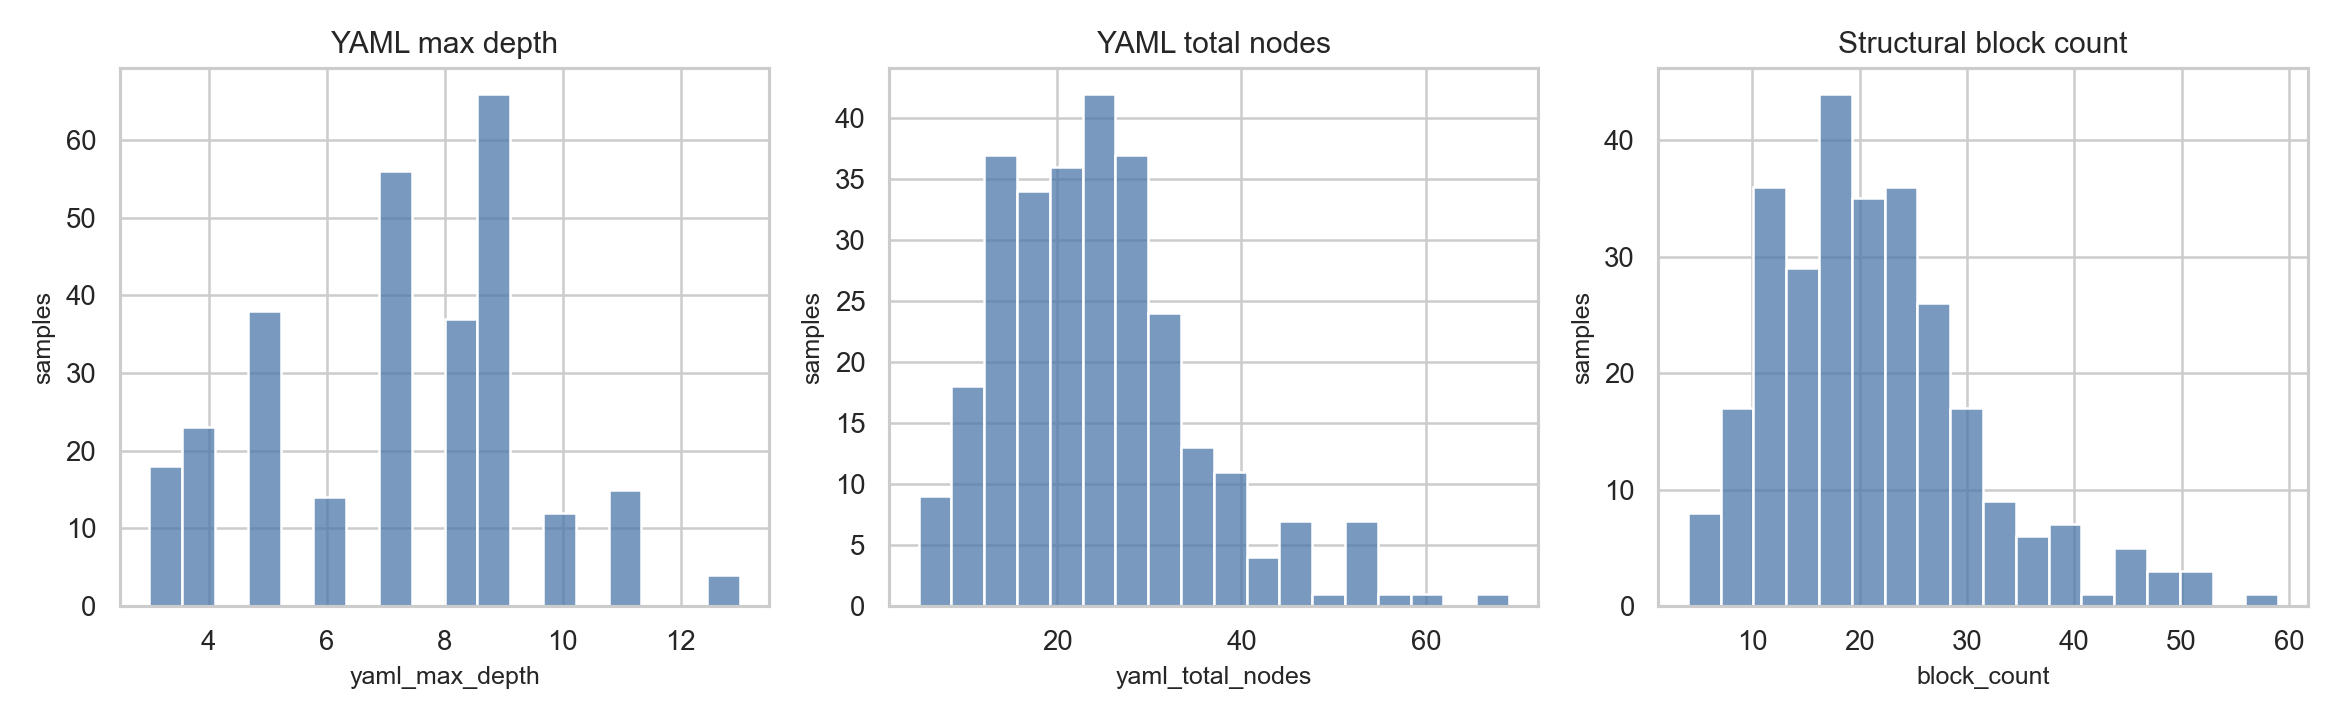
\includegraphics[width=0.82\textwidth]{figures/chapter3/complexity_histograms.png}
\caption{Distribuciones de complejidad estructural en el dataset canónico.}
\label{fig:ch3_complexity_hist}
\end{figure}

\begin{figure}[htbp]
\centering
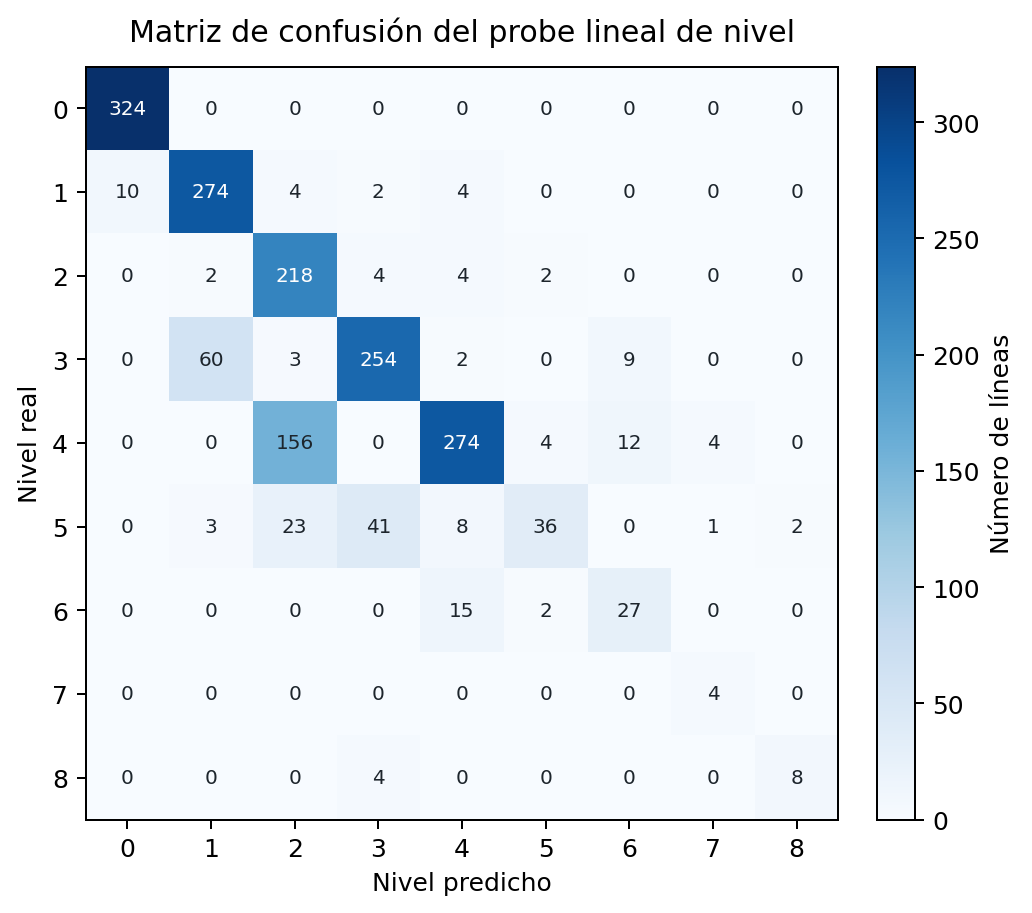
\includegraphics[width=0.70\textwidth]{figures/chapter3/confusion_matrix_validation_line_first_token__linear.png}
\caption{Matriz de confusión del \textit{latent probe} para predicción de nivel de indentación.}
\label{fig:ch3_probe_confusion}
\end{figure}

\subsection{Heterogeneidad estructural por tipo de recurso}

Diferentes tipos de Kubernetes tienen ``firmas'' estructurales muy distintas. Un ConfigMap es una estructura plana: contiene solo claves y valores al nivel 1 bajo el
campo \texttt{data}, lo que produce anidamiento de profundidad 3 - 4. Un Secret es similar. Por el contrario, un Deployment o StatefulSet introduce templating: el campo
\texttt{spec} contiene un \texttt{template}, que a su vez contiene otro \texttt{spec} para los pods, que contiene \texttt{containers}, que contiene \texttt{volumeMounts}.
Esto produce anidamiento de profundidad 8 - 10 o más.

Esto significa que la dificultad estructural no es uniforme: cuando el modelo ve un Pod, tiene muchas más muestras de anidamiento profundo que cuando ve un ConfigMap.
En este sentido, el sesgo de frecuencia en el dataset (Pod y DaemonSet dominan con 33\% del total) está correlacionado con una mayor complejidad estructural. Esto es un
matiz importante: no es que el modelo tenga sesgo hacia tipos simples (que sería un problema de falta de cobertura), sino que ha visto muchos ejemplos de
estructuras complejas.

\subsection{Presencia de campos semánticos}

Algunos campos Kubernetes son obligatorios en todos los manifiestos (como \texttt{metadata}), mientras que otros son opcionales y aparecen solo en ciertos tipos de recursos.
Analizando el dataset:

\begin{itemize}
\item \texttt{metadata}: presente en el 100\% de los manifiestos (requerida por la API)
\item \texttt{spec}: presente en el 86.2\% (casi todos excepto Namespace y algunos objetos triviales)
\item \texttt{containers}: presente en el 64.7\% (Pods, Deployments, y otros workloads)
\item \texttt{image}: presente en el 64.7\% (corolario de containers)
\item \texttt{ports}: presente en el 21.2\% (Services, Ingresses, algunos Pods)
\item \texttt{volumes}: presente en el 13.4\% (solo algunos workloads)
\item \texttt{env}: presente en el 7.77\% (algunas aplicaciones con configuración)
\end{itemize}

\begin{figure}[htbp]
\centering
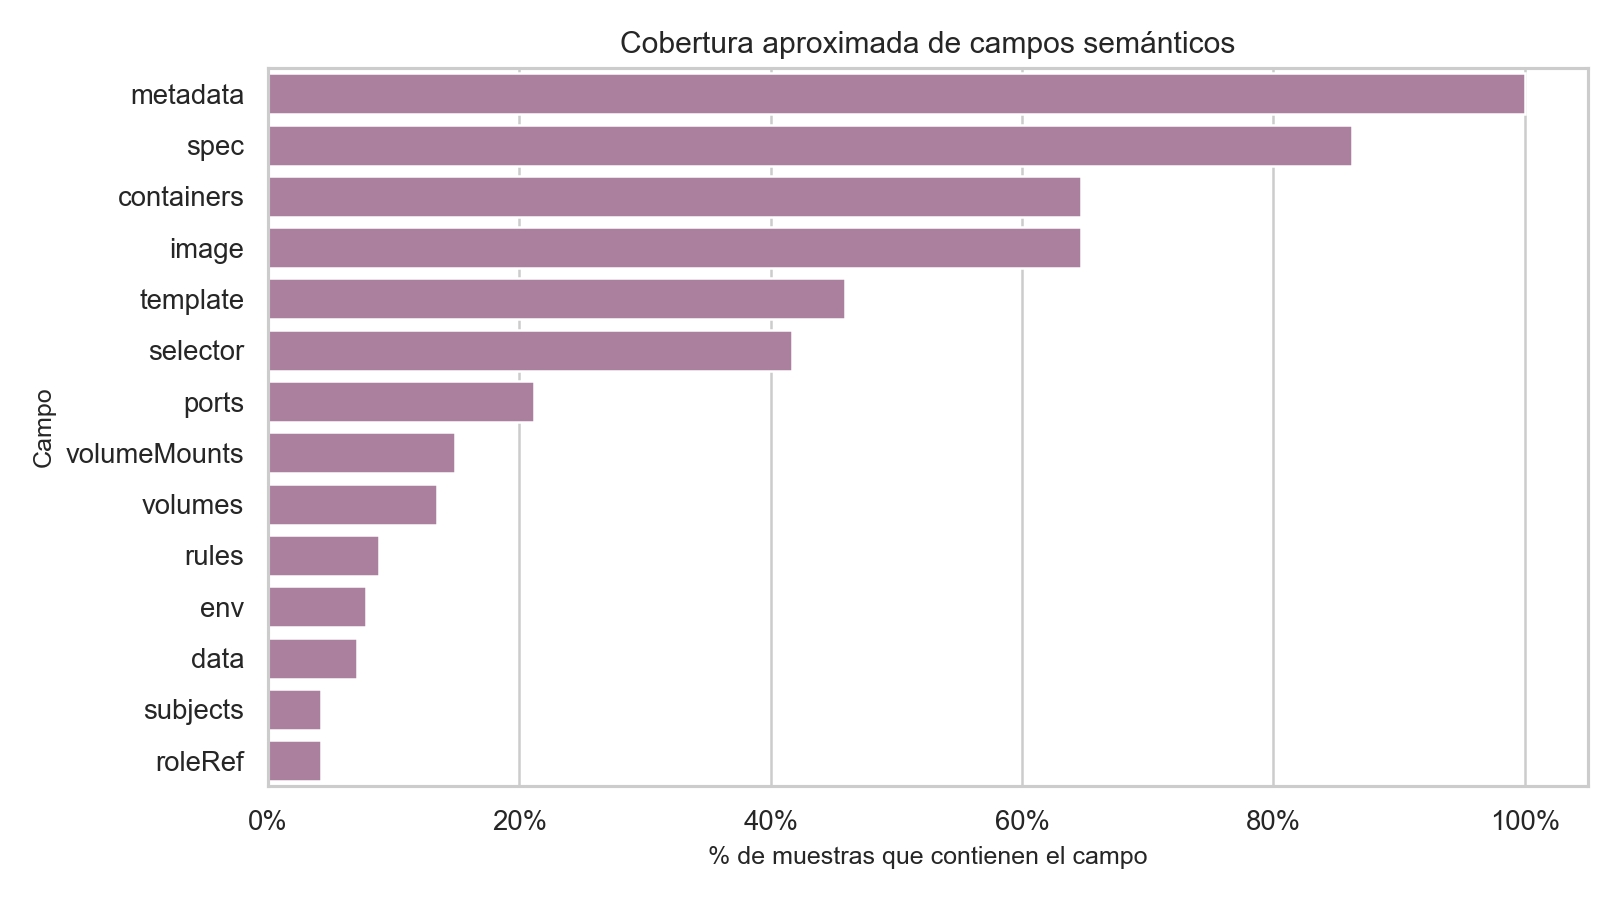
\includegraphics[width=0.8\textwidth]{figures/chapter3/semantic_field_presence.png}
\caption{Cobertura de campos semánticos relevantes en manifiestos Kubernetes del dataset.}
\label{fig:ch3_semantic_fields}
\end{figure}

\noindent Esta distribución refleja la naturaleza del dominio: la mayoría de manifiestos son workloads (Pods, Deployments, etc.) que necesitan \texttt{spec} y \texttt{containers},
pero una minoría significativa son recursos de configuración o red con campos mucho más específicos. La implicación para el modelo es que debe aprender patrones estructurales
de alta varianza: a veces \texttt{spec} contiene containers, a veces contiene replicas, a veces contiene selector.

\section{Análisis de los prompts}

\subsection{Variantes y longitud}

Como ya se ha visto, cada muestra tiene asociados dos prompts: una versión más descriptiva (\textit{question}) y una versión simplificada (\textit{simplified}). El
objetivo es capturar la robustez
del sistema ante diferentes formas de expresar la misma especificación. La versión question tiene una longitud mediana de 54 palabras, con máximo de 176. La versión
simplified
tiene mediana de 36 palabras, con máximo de 139.

En cuanto a tokens del tokenizador del modelo base (Qwen 2.5 - 7B), los prompts question tienen longitud mediana de aproximadamente 45 tokens, mientras que simplified tiene
mediana de 27 tokens. La diferencia entre conteo de palabras y conteo de tokens es importante porque ciertos identificadores de Kubernetes (como nombres en camelCase o paths)
se tokenizan de forma subóptima, fragmentándose en múltiples tokens. Esto aumenta la longitud efectiva del prompt para el modelo respecto a lo que el conteo de palabras sugeriría.

\begin{figure}[htbp]
\centering
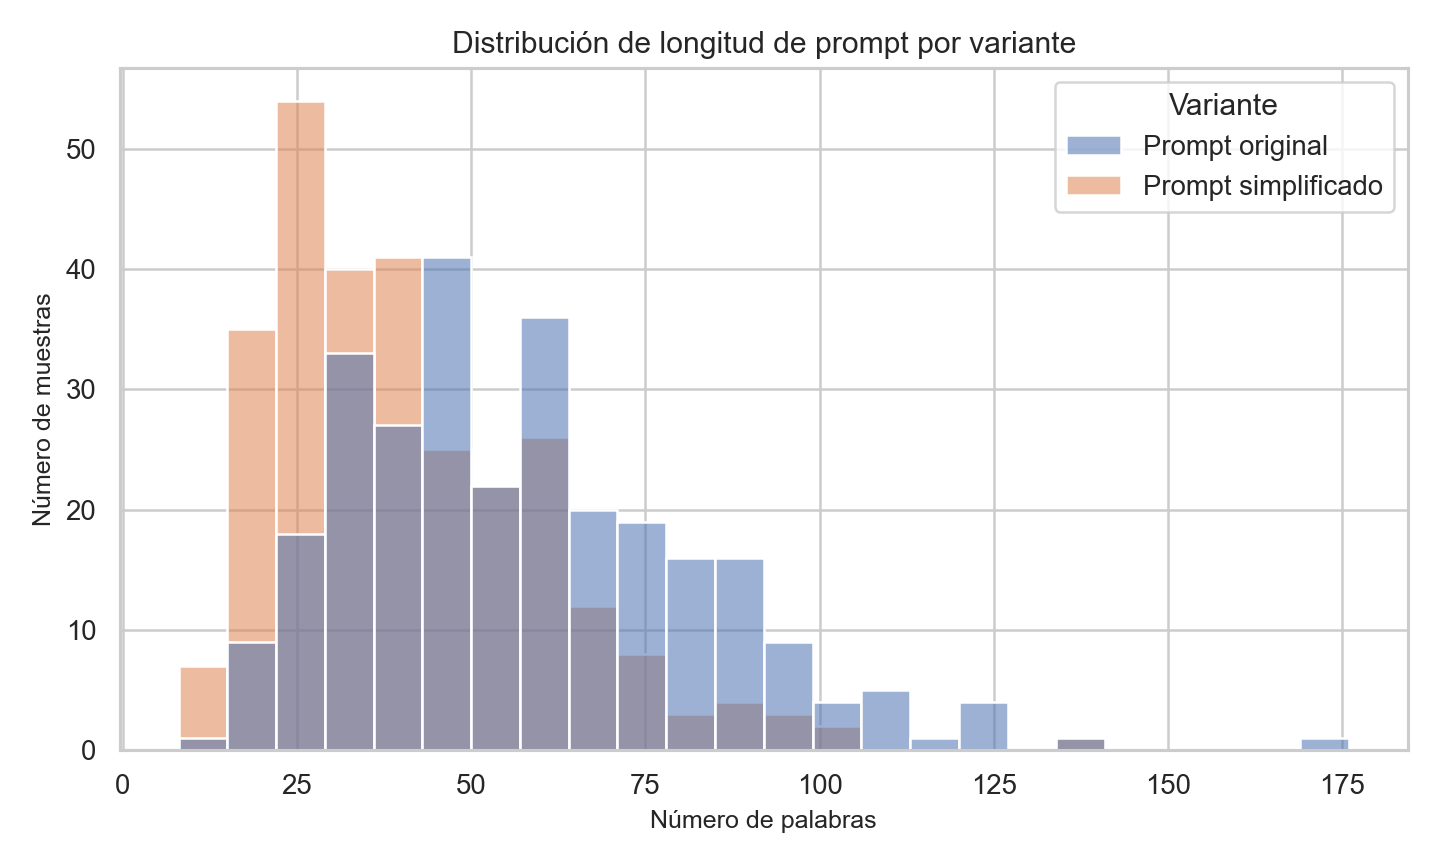
\includegraphics[width=0.78\textwidth]{figures/chapter3/prompt_length_distribution.png}
\caption{Distribución de longitud de prompt por variante (\textit{question} y \textit{simplified}).}
\label{fig:ch3_prompt_length}
\end{figure}

\subsection{Similitud entre variantes}

La similitud semántica entre el prompt question y el prompt simplified se mide mediante similitud coseno entre embeddings de frase. Si \(\mathbf{e}_q\) y \(\mathbf{e}_s\) representan los embeddings de las variantes \textit{question} y \textit{simplified}, respectivamente, la medida utilizada es:

\[
\operatorname{sim}(q,s) =
\frac{\mathbf{e}_q^\top \mathbf{e}_s}
{\|\mathbf{e}_q\|_2\,\|\mathbf{e}_s\|_2}.
\]

En el dataset, esta similitud varía sustancialmente: el rango va de 0.02 a 1.0,
con mediana de 0.68. Esto indica que para algunas muestras, ambas variantes son casi idénticas (casos donde simplificar no aporta casi nada), mientras que para otras, la versión
simplificada omite detalles cruciales. Un caso extremo sería un prompt que especifica detalles sobre tolerancias de nodos cuya versión simplificada solo menciona ``pod con
restricciones'', capturando la esencia pero perdiendo especificidad.

\begin{figure}[htbp]
\centering
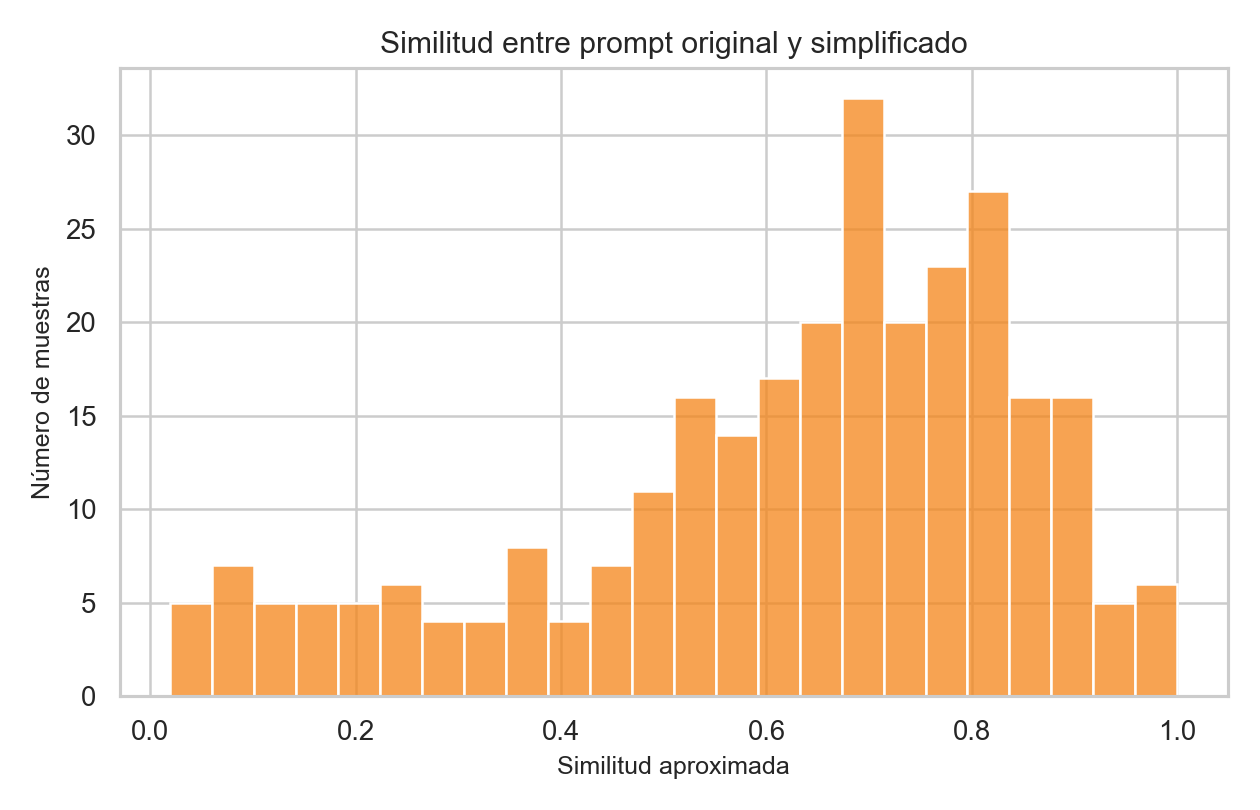
\includegraphics[width=0.78\textwidth]{figures/chapter3/prompt_pair_similarity.png}
\caption{Similitud semántica entre variantes de prompt por muestra.}
\label{fig:ch3_prompt_similarity}
\end{figure}

\subsection{Requisitos capturados}

De los prompts se pueden extraer requisitos semánticos mediante patrones de regex: tipo de recurso (Pod, Deployment, etc.), nombres de aplicación, imágenes de contenedor,
labels,
puertos expuestos, número de replicas, volúmenes y mounts, variables de entorno, namespaces, y restricciones de scheduling (afinidad, tolerancias, etc.). Esta lectura de
la salida
respecto a requisitos expresados en lenguaje natural sigue la línea de otras evaluaciones evaluaciones que separan validez técnica y adecuación a la intención
\citep{ueno2024migrating, xu2024cloudevalyaml}. El grado en que estos
requisitos aparecen explícitamente en el prompt varía. Algunos prompts especifican casi todos los requisitos; otros proporcionan solo los campos esenciales.
Y de estos requisitos
mencionados en el prompt, no todos aparecen en el manifiesto YAML de referencia. Un prompt puede especificar ``el contenedor debe ejecutarse como usuario no-root'',
pero el manifiesto
del dataset podría no incluir la sección \texttt{securityContext}, bien porque fue omitido deliberadamente o porque el contexto del dataset no cubre todos los requisitos
mencionados.

De esta extracción de requisitos se construyen métricas de cobertura semántica, que permiten evaluar no solo si el manifiesto es sintácticamente correcto,
sino si cumple con
los requisitos explícitos del prompt. Por ejemplo, si el prompt menciona un puerto específico, ¿está ese puerto presente en el manifiesto generado? Si el prompt
especifica un número 
de replicas, ¿coincide con el valor en el YAML? Esto evita depender de métricas como BLEU o ROUGE, que no capturan adecuadamente la corrección semántica
en este dominio cuando la salida es un artefacto técnico validable \citep{chen2021evaluating, xu2024cloudevalyaml}.

\subsection{Correlación entre longitud y complejidad}

Un aspecto relevante es si prompts más largos producen manifiestos más complejos. Existe una correlación positiva moderada entre la longitud del prompt (en palabras o tokens) y
la complejidad del manifiesto, medida como número de líneas (\texttt{block\_count}) o número de nodos en el árbol parseado (\texttt{yaml\_total\_nodes}). Sin embargo,
la correlación no es perfecta: hay prompts relativamente breves que generan manifiestos complejos
(por ejemplo, ``crea un Deployment'' en un contexto donde Deployment implica naturalmente múltiples contenedores y volúmenes) y prompts largos con manifiestos simples (por ejemplo,
explicaciones verbosas de un ConfigMap simple).

\begin{figure}[htbp]
\centering
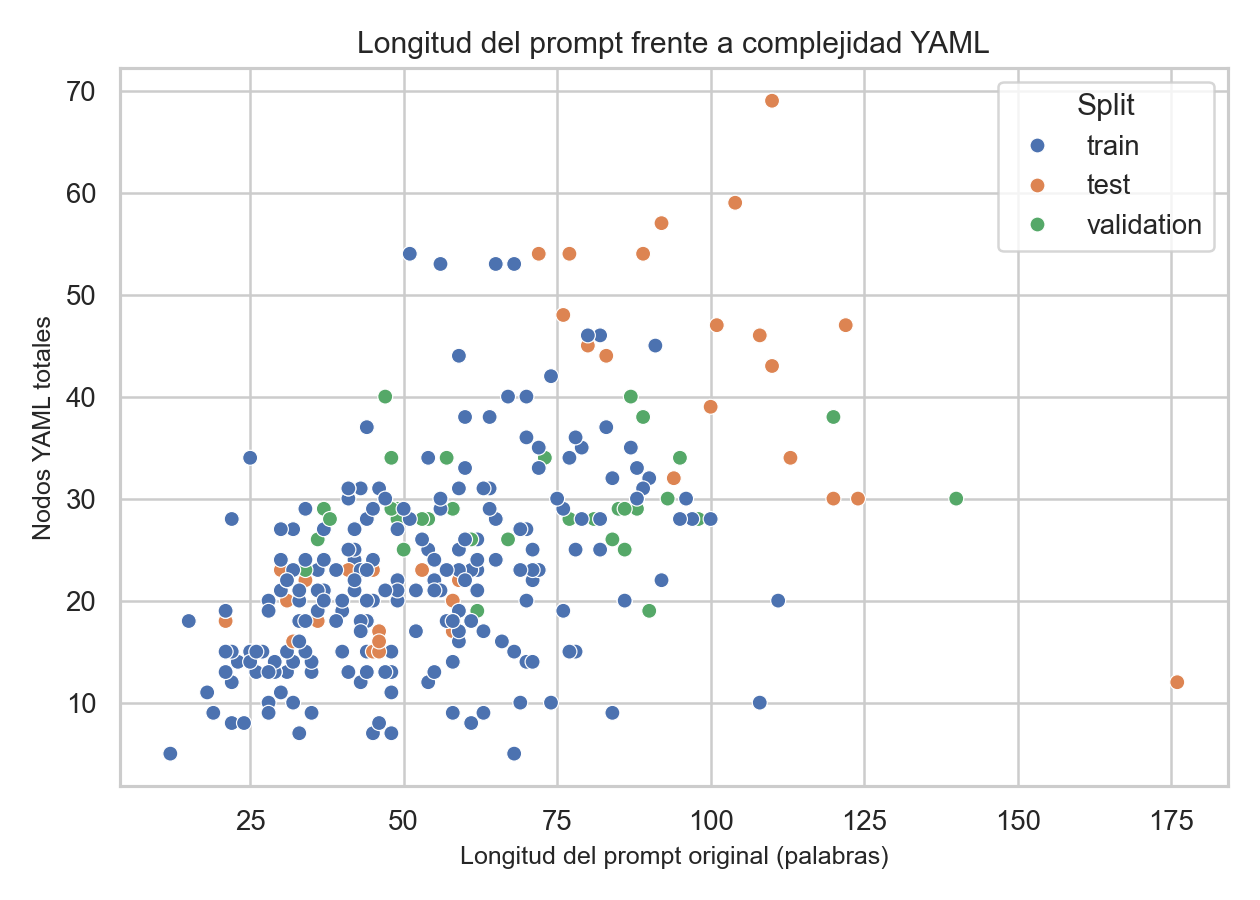
\includegraphics[width=0.78\textwidth]{figures/chapter3/prompt_length_vs_yaml_nodes.png}
\caption{Relación entre longitud de prompt y complejidad estructural del YAML.}
\label{fig:ch3_prompt_vs_complexity}
\end{figure}

\section{Observaciones con implicaciones de diseño}

El análisis anterior revela patrones del dataset que tienen consecuencias directas para cómo el modelo aprende a generar manifiestos. En esta sección se contrastan estas
observaciones con los resultados experimentales.

\subsection{La pared del nivel 5}

El dataset tiene <8\% de bloques en niveles de indentación $\geq 5$. En términos de la distribución anterior, esta región profunda se resume como:

\[
p_{\geq 5} = \sum_{k=5}^{8} p_k.
\]

\subsection{Anti-patrones de seguridad presentes en los datos de entrenamiento}

Los manifiestos del dataset no son perfectos desde el punto de vista de seguridad. El análisis realizado detecta varios anti-patrones en las salidas generadas, muchos de
los cuales
están presentes también en los objetivos de los datos de entrenamiento:

\begin{itemize}
\item Ausencia de \texttt{resources.requests} y \texttt{resources.limits}: 261 ocurrencias en 70 muestras (3.7 por muestra en promedio)
\item Ausencia de \texttt{runAsNonRoot} en \texttt{securityContext}: 71 ocurrencias
\item Ausencia de \texttt{readOnlyRootFilesystem}: 71 ocurrencias
\item Uso de tag \texttt{latest} de imagen o ausencia de tag específico: 67 ocurrencias
\item Otras incidencias menores: volúmenes sin montajes correspondientes, etc.
\end{itemize}
